\chapter{Background}
\label{cap:nomePrimoCapitoloTesi}
\lhead{\textbf{\rightmark}}
\section{Melanoma}
\indent{
Il melanoma cutaneo è un tumore che deriva dalla trasformazione tumorale dei melanociti, alcune delle cellule che formano la pelle. La pelle è l'organo più esteso del nostro corpo ed è formata da tre strati: l'epidermide, il derma e il tessuto sottocutaneo o grasso. I melanociti fanno parte, insieme ai cheratinociti, dell'epidermide e hanno il compito di produrre melanina, un pigmento che protegge dagli effetti dannosi dei raggi solari. In condizioni normali i melanociti possono dar luogo ad agglomerati scuri visibili sulla superficie della pelle e noti come nei (\textbf{nevi} è il termine medico). \cite{melanomi1}
\begin{figure}[h]
	\begin{center}     
		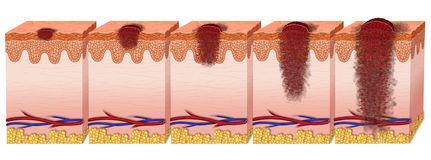
\includegraphics[scale=0.90]{figure/capitolo1/melanoma.jpg}
	\end{center}
	\caption{Melanoma}	
\end{figure}
Il melanoma cutaneo è piuttosto raro nei bambini e colpisce soprattutto attorno ai 45-50 anni, anche se l'età media alla diagnosi si è abbassata negli ultimi decenni.
\newline
In Italia, i dati AIRTUM 2017 (Associazione italiana registri tumori) stimano circa 7.300 nuovi casi ogni anno tra gli uomini e 6.700 tra le donne. L’incidenza è in continua crescita ed è addirittura raddoppiata negli ultimi 10 anni.\cite{2}
\newline
È opportuno ricordare che il melanoma cutaneo rappresenta solo una piccola percentuale (circa il 5 per cento) di tutti i tumori che colpiscono la pelle.
\subsection{Come si forma un Melanoma}
Un \textit{melanoma} inizia nelle cellule della pelle chiamate melanociti. I melanociti sono le cellule che producono la melanina, che conferisce alla pelle il suo colore. La melanina protegge anche gli strati più profondi della pelle dai dannosi raggi ultravioletti (UV) del sole. Quando le persone sono esposte alla luce del sole, i melanociti producono più melanina e inducono la pelle ad abbronzarsi, questo accade anche quando la pelle è esposta ad altre forme di luce ultravioletta (come in una cabina abbronzante). 
\newline
Se la pelle riceve la luce ultravioletta, i melanociti possono iniziare a crescere in modo anomalo e diventare cancerogeni. Questa condizione chiamata melanoma, come mostrato nella Figura 1.1, il cancro del melanoma cresce nello strato esterno dove i melanociti si trovano sulla pelle, quindi in una fase successiva si diffonde ad altre parti del corpo come ossa e polmoni.
\newline
Pertanto, il melanoma è letale se non rilevato nella fase iniziale; questa consapevolezza ha portato ad aumentare l'interesse delle soluzioni diagnostiche in fase iniziale.
Il problema della ricerca di soluzioni per il rilevamento del melanoma in fase iniziale diventa sempre più importante, in un periodo storico in cui il melanoma maligno sta aumentando rapidamente in tutto il mondo, anche nei paesi con tassi di incidenza storicamente bassi, e questo aumento si sta verificando a un ritmo sempre più veloce rispetto a qualsiasi altra neoplasia, le strategie basate sulla popolazione per controllare la malattia si sono concentrate principalmente sulla prevenzione primaria e sulla diagnosi precoce.
\subsection{Approcci e metodi per il riconoscimento}
Per l'identificazione dei melanomi, i dermatologi consigliano di utilizzare  la "\textit{regola ABCDE}" (A = asimmetria, B = irregolare
bordi, C = colore, D = dimensione, E = evoluzione).
\begin{itemize}
	\item A - asimmetria: metà di un nevo non corrisponde all'altra.
	\item B - bordi: i bordi sono irregolari, irregolari, dentellati o sfocati.
	\item C - colore: il colore non è lo stesso dappertutto e può includere sfumature di marrone o nero, o anche macchie di rosa, rosso, bianco o blu.
	\item D - dimensione/diametro: quando il diametro è un valore maggiore di 6 millimetri
	\item E - evoluzione: il nevo sta cambiando di dimensione, forma o colore
\end{itemize}
\begin{figure}[h]
	\begin{center}     
		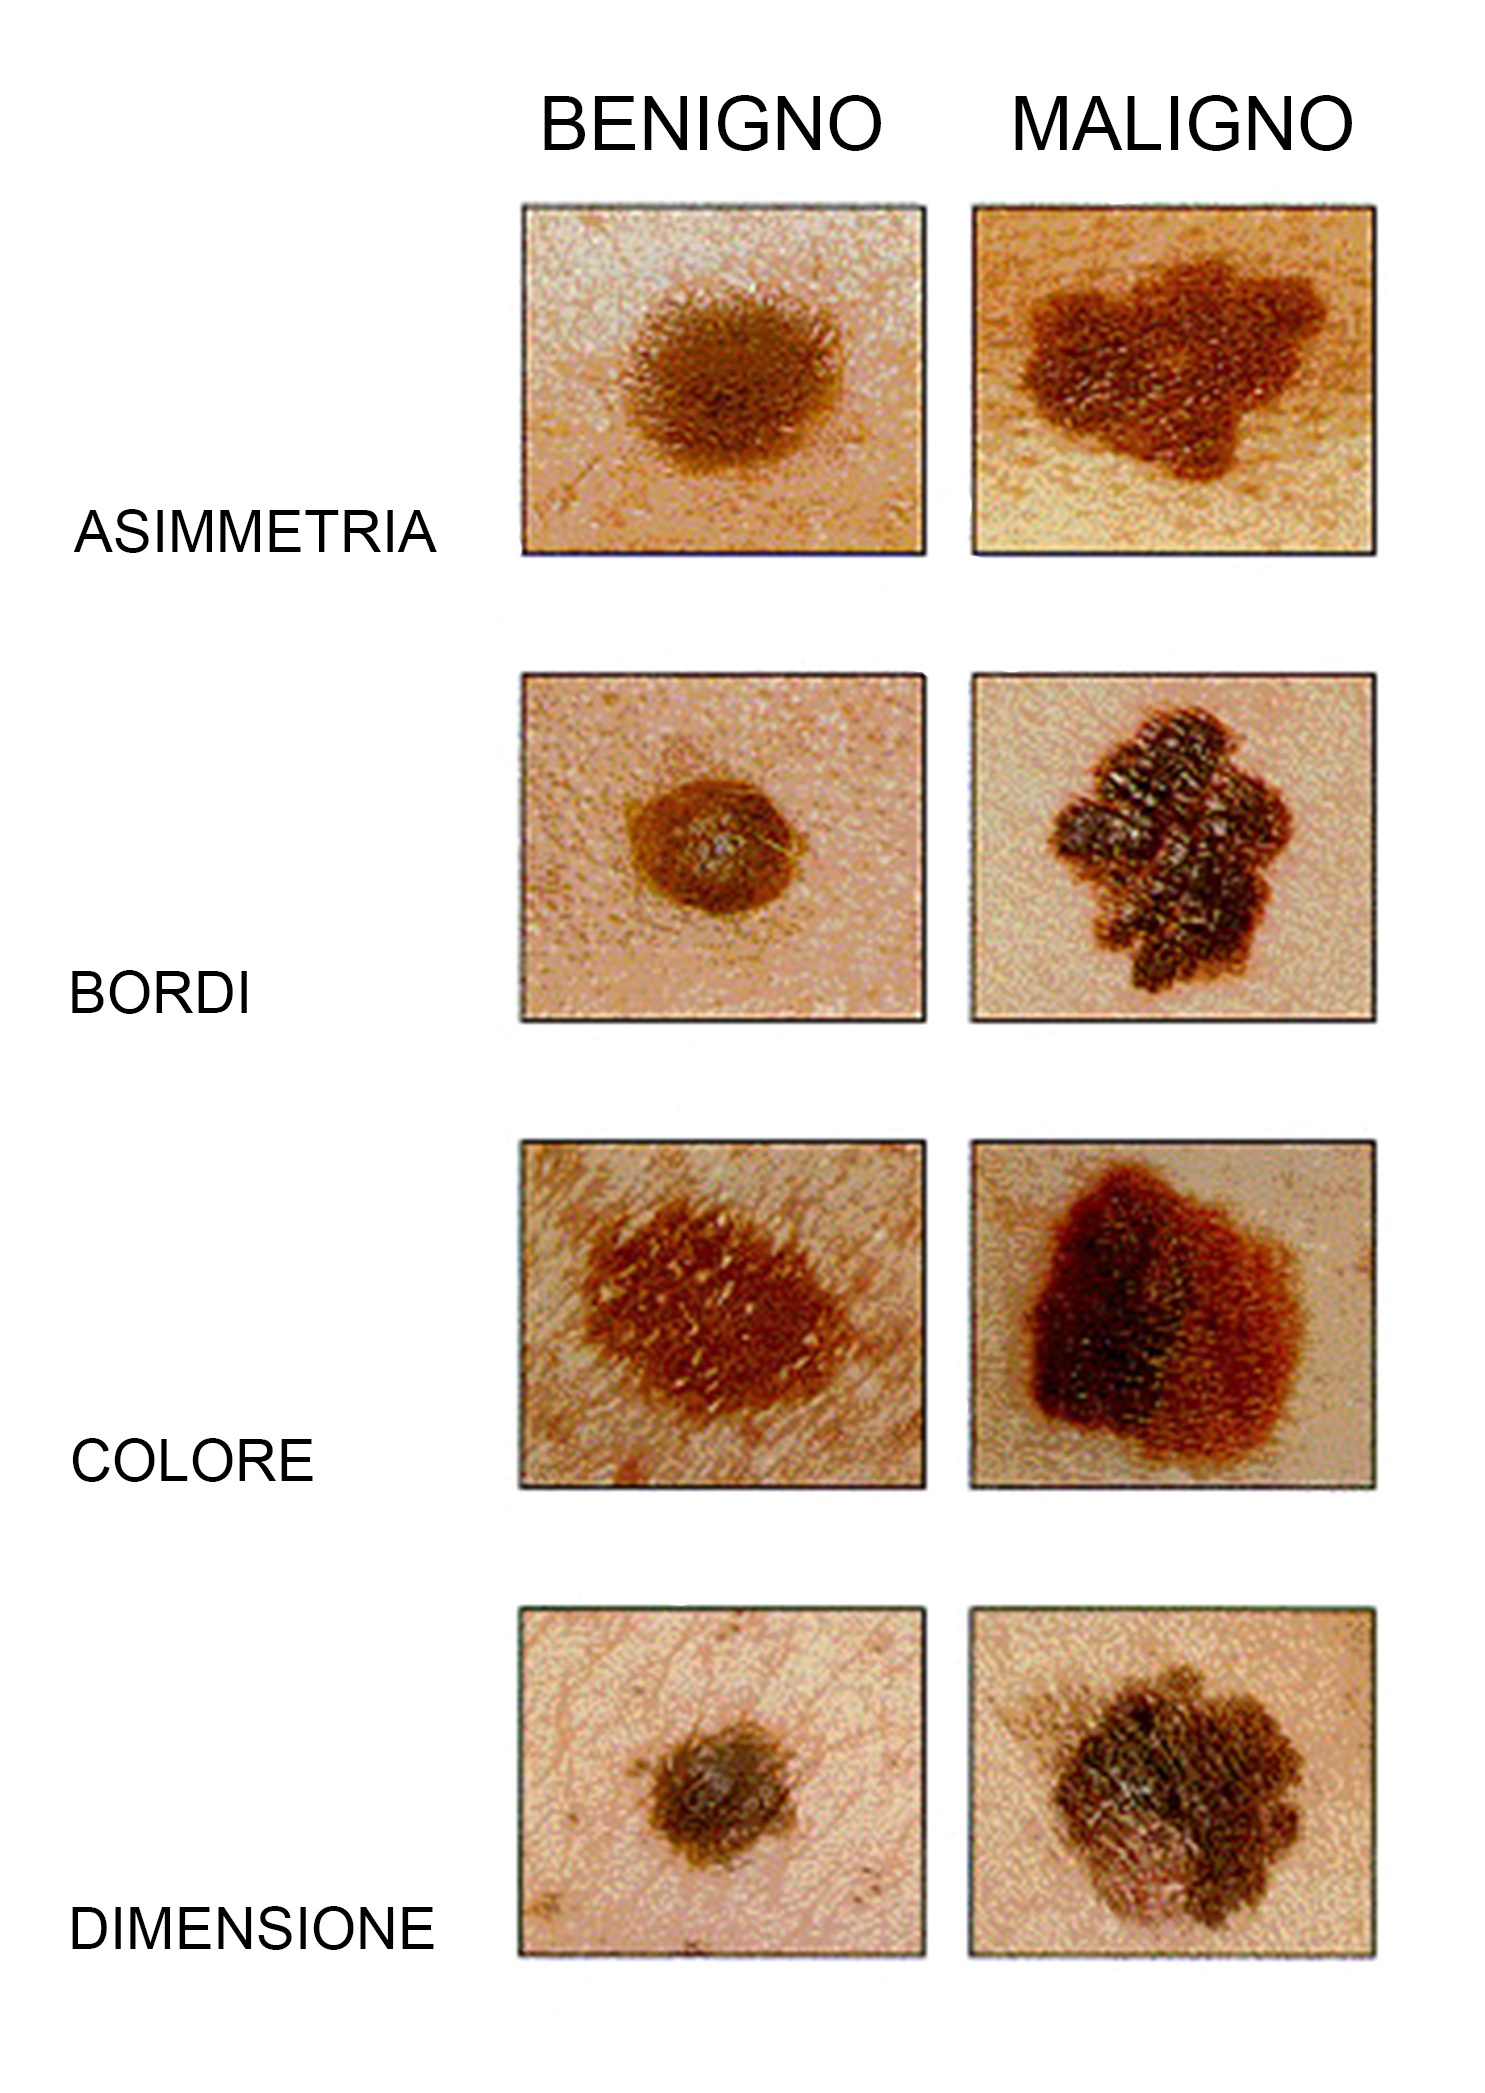
\includegraphics[scale=0.50]{figure/capitolo1/classificazione.jpg}
	\end{center}
	\caption{ABCD Features}	
\end{figure}
Il melanoma può essere confuso con altre lesioni benigne e la diagnosi differenziale si svolge osservando il colore (più intenso di
 altri nevi dello stesso soggetto), l'età di esordio (più tardi
rispetto agli altri nevi), il raddoppio della taglia in 6-8 mesi.
\newline
Forma piatta palpabile o lesione leggermente rilevata sulla pelle.
\newline
Negli ultimi vent'anni sono stati proposti sistemi di diagnosi assistita per i dermatologi, da computer basati sulla visione artificiale nella diagnosi precoce del melanoma.
 Però, questi sistemi sfruttano solo un insieme ridotto di parametri o implementano un classificatore del melanoma che cerca di sostituire i dermatologi senza supportare la loro esperienza in
classificazione delle lesioni cutanee.
\newline
L'obiettivo di questa tesi è quello di fornire al dermatologo un'assistenza all'analisi dei nevi in realtà aumentata, offrendo anche un classificatore che aiuterà il dermatologo a stabilire se il nevo può essere o meno un melanoma, ma con l'obiettivo di estrarre quante più informazioni possibili in tempo reale e visibili in realità aumentata.
\newpage
\section{Reti Neurali}
Le reti neurali sono un potente strumento utilizzato nel campo dell'intelligenza artificiale.
In realtà le reti neurali, nonostante abbiano avuto la loro esplosione negli ultimi anni, non sono per nulla recenti; il primo modello di neurone artificiale è infatti stato proposto nel 1943, negli anni successivi ci sono stati ulteriori studi e miglioramenti tra cui il modello del percettore da parte di Rosenblatt, fra gli anni '50 e gli anni '60. 
Il grande limite delle reti neurali è sempre stata la mancanza di prestazioni computazionali lato hardware che consentisse l'esecuzione di queste reti, infatti le reti neurali venivano considerate complicate e costose in termini computazionali.
\newline
L'avvento del \textit{Deep Learning} verso la fine degli anni 2000, ha portato un forte e rinnovato interesse per queste reti. \cite{maiani2016applicazioni}
\newline
\subsection{Deep Learning}
Il \textit{deep learning} è un campo di studio dell'intelligenza artificiale (AI) che consente ai sistemi di apprendere e migliorare automaticamente senza l'ausilio umano. Si concentra, in particolar modo, sullo sviluppo di applicazioni che riescono ad acquisire dati e costruire modelli che riescono a prendere decisioni in base ai dati osservati.
\newline
In base alla modalità di apprendimento adottato, i metodi di apprendimento automatico sono generalmente classificati come supervisionati o non supervisionati. Nell'apprendimento supervisionato, un modello viene costruito su determinati dati insieme alle rispettive etichette. 
\newline
Nell'apprendimento senza supervisione, invece, le etichette precedenti sono inaccessibili o accessibili ma non importanti per l'applicazione d'interesse.
Quest'ultimo, quindi, consiste nello studio di come i sistemi possano dedurre funzioni per definire strutture nascoste da dati non etichettati.
\newline
L'apprendimento semi-supervisionato è un'altra direzione il cui scopo è sfruttare i dati di un'etichetta di piccole dimensioni e dati senza etichetta di grandi dimensioni.
Uno sguardo ravvicinato alla letteratura recente direbbe che un grande focus è orientato al deep learning.
\newline
A differenza delle \textit{reti neurali tradizionali}, vari livelli di neuroni nell'apprendimento profondo eseguono un apprendimento gerarchico della rappresentazione dei dati tramite trasformazioni non lineari. In altre parole, i dati vengono passati cumulativamente attraverso una lunga catena di livelli (quindi, la descrizione profonda), dove ogni strato può essere completamente o parzialmente connesso a quello precedente.
\newpage
\subsection{Reti Neurali Convoluzionali}
Le reti neurali convoluzionali (CNN) sono di fatto delle reti neurali artificiali, ispirati a processi biologici e progettate per riconoscere modelli direttamente da immagini pixel (o altri segnali), incorporando sia l'estrazione delle caratteristiche che la classificazione.
\newline
Una tipica CNN coinvolge quattro tipi di livelli: convoluzionale, attivazione, pooling e completamente connessi (noti anche come densi). 
\newline
Uno strato convoluzionale è caratterizzato da una scarsa connettività locale, in cui ogni neurone dello strato è collegato solo ad una piccola area locale dell'input, che assomiglia al campo ricettivo nel sistema visivo umano.
\newline
I livelli di pooling riducono la sensibilità dell'output a piccoli spostamenti di input. Infine, vengono posti uno o più strati densi, ciascuno seguito da uno strato di attivazione, che producono il risultato della classificazione. La formazione delle CNN viene eseguita in modo simile a quella di altre ANN. \cite{anthimopoulos2016lung}

\section{Realtà Aumentata}
Le origini di questa tecnologia risalgono al 1901, in letteratura, in un romanzo di Frank L.Baum: "The Master Key", dove un ragazzino entra in possesso di occhiali modernissimi per l'epoca in grado di capire se le persone fossero buone o cattive attraverso una lettera\footnote{character marker} sul capo della persona che mostrava il tipo di persona.\cite{baum1901master}
\newline
\newline
La Realtà Aumentata, ad oggi, viene utilizzata in molti ambiti. Uno su tutti è lo sviluppo di applicazioni per smartphone.
\newline
Le aree di interesse della AR sono molteplici: videoludico, turistico, medico, educativo, architettonico.
\newline
La possibilità di creare oggetti virtuali in ambienti reali è di estrema utilità per la vendita di prodotti come automobili, mobili, e col tempo sta diventando un supporto sempre più richiesto in ambito medico. \cite{garofalo}

}
